\documentclass[12pt]{article}
\usepackage[utf8]{inputenc}
\usepackage{polski}
\usepackage{listings}
\usepackage{amsmath}
\usepackage{multicol}
\usepackage{graphicx}
\graphicspath{ {./images/} }
\title{
	Obliczenia naukowe \\
	Sprawozdanie 2
}
\lstset{
basicstyle=\small\ttfamily,
breaklines=true
}
\addtolength{\oddsidemargin}{-.5in}
\addtolength{\evensidemargin}{-.5in}
\addtolength{\textwidth}{1.75in}
\addtolength{\topmargin}{-.7in}
\addtolength{\textheight}{1.75in}

\date{7 listopada 2019}
\author{Józef Piechaczek}

\begin{document}

\pagenumbering{gobble}
\maketitle
\newpage
\pagenumbering{arabic}

\setlength{\abovedisplayskip}{5pt}
\setlength{\belowdisplayskip}{5pt}

\section{Zadanie 1}
Zadanie 1 polega na ponownym przeprowadzeniu eksperymentu z listy 1 dla zadania 5. Zadanie to polega na obliczeniu iloczynu skalarnego dwóch wektorów, przy czym obcięte są dwie ostatnie cyfry przy wartości $x_4$ oraz $x_5$. Wektory po obcięciu wyglądają następująco:
\begin{align*}
	x &= [2.718281828,-3.141592654,1.414213562,0.577215664,0.301029995] \\
	y &= [1486.2497,878366.9879,-22.37492,4773714.647,0.000185049]
\end{align*}
Iloczyn należy policzyć za pomocą czterech algorytmów
\begin{enumerate}
	\item w przód
	\item w tył
	\item od największego do najmniejszego
	\item od najmniejszego do największego
\end{enumerate}

Wyniki eksperymentu przedstawia poniższa tabela:
\begin{table}[h!]
	\small
	\centering
    \label{tab:table1}
    \begin{tabular}{|c|c|c|c|c|}
    		\hline
      	 & \multicolumn{2}{c|}{Float32} & \multicolumn{2}{c|}{Float64}\\
      	\hline
      	 & $x_1 \cdot y$ & $x_2 \cdot y$  & $x_1 \cdot y$ & $x_2 \cdot y$ \\
      	\hline
      	1 & -0.4999443 & -0.4999443 & 1.0251881368296672e-10 & -0.004296342739891585\\
		\hline
      	2 & -0.4543457 & -0.4543457 & -1.5643308870494366e-10 & -0.004296342998713953\\
		\hline
      	3 & -0.5 & -0.5 & 0.0 & -0.004296342842280865\\
		\hline
      	4 & -0.5 & -0.5 & 0.0 & -0.004296342842280865\\
		\hline
    \end{tabular}
\end{table}

\subsubsection*{Wnioski:}
Patrząc na tabelę możemy zauważyć, że wartości dla \textbf{Float32} nie uległy zmianie dla żadnego z algorytmów. Wynika to z faktu iż 


\section{Zadanie 2}
Zadanie 2 polega na narysowaniu wykresu funkcji $f(x) = e^x*ln(1+e^{-x})$ w co najmniej dwóch dowolnych programach do wizualizacji oraz na policzeniu granicy $ \lim_{x \to \infty} f(x)$.

\newpage
\subsubsection*{Wykresy:}

\begin{figure}[!htb]
\minipage{0.49\textwidth}
  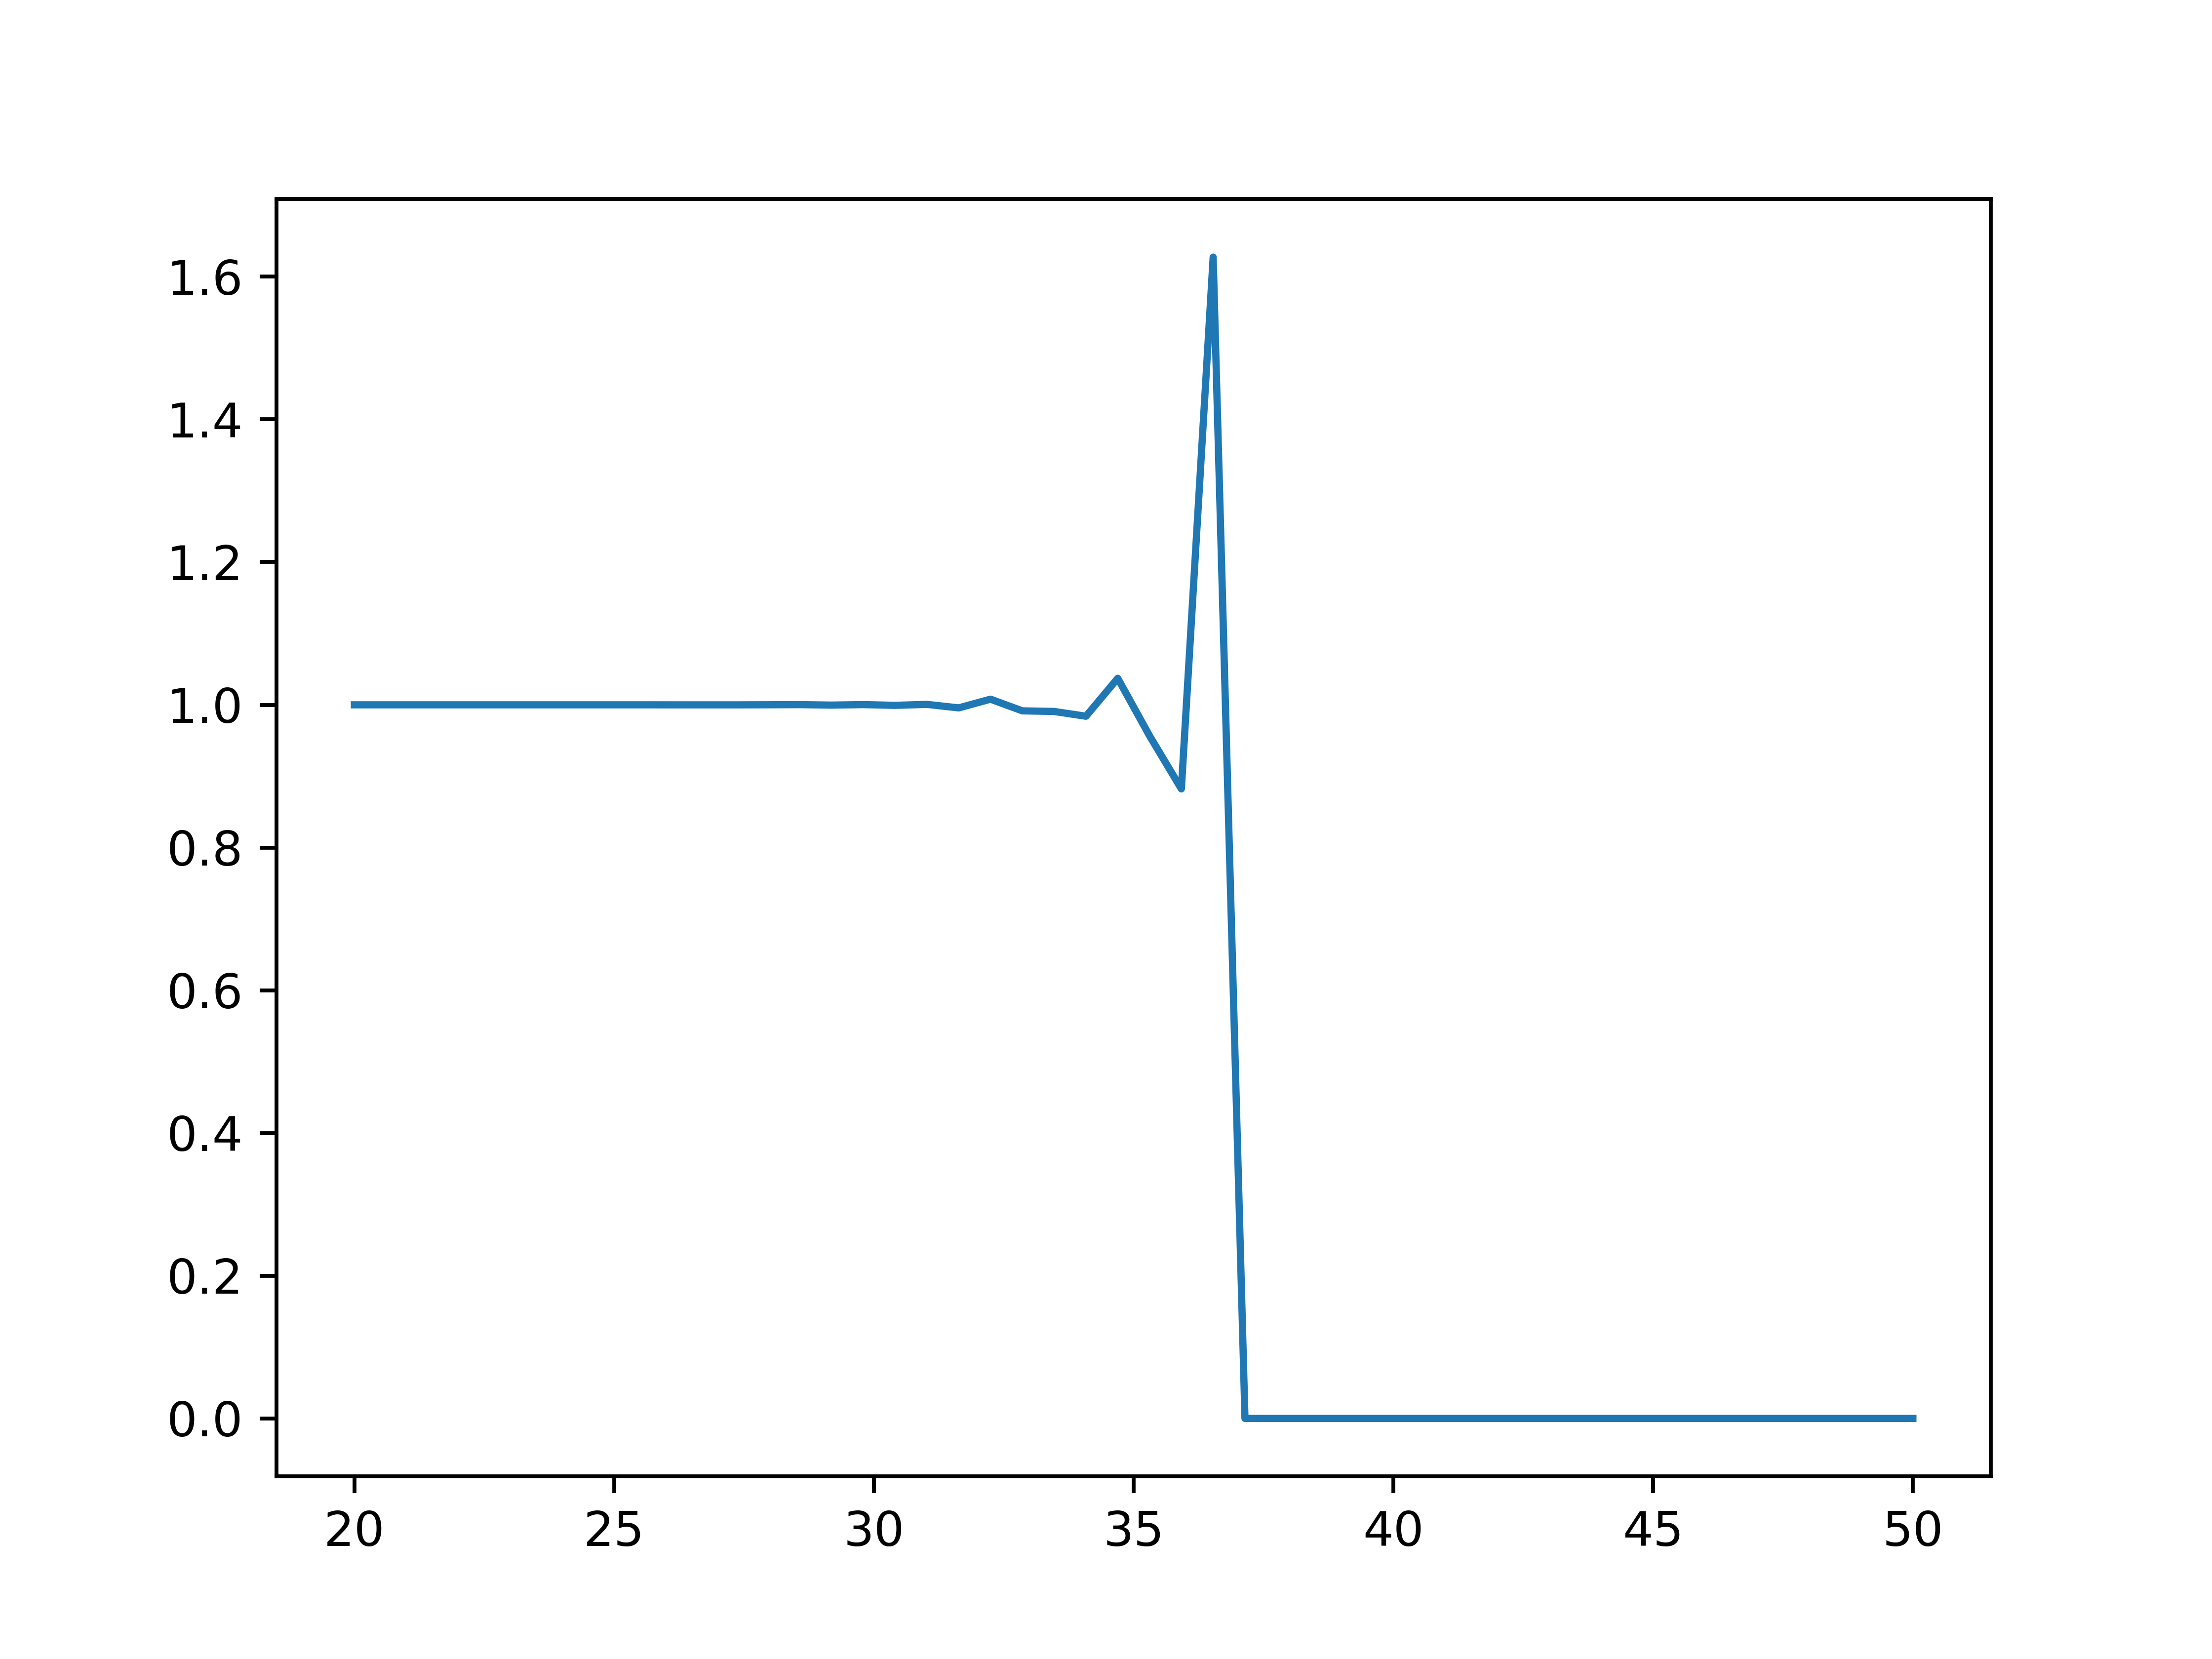
\includegraphics[width=\linewidth]{zad2_plot_py2.png}
  \caption{PyPlot od 20 do 50}\label{fig:figure1}
\endminipage\hfill
\minipage{0.49\textwidth}
  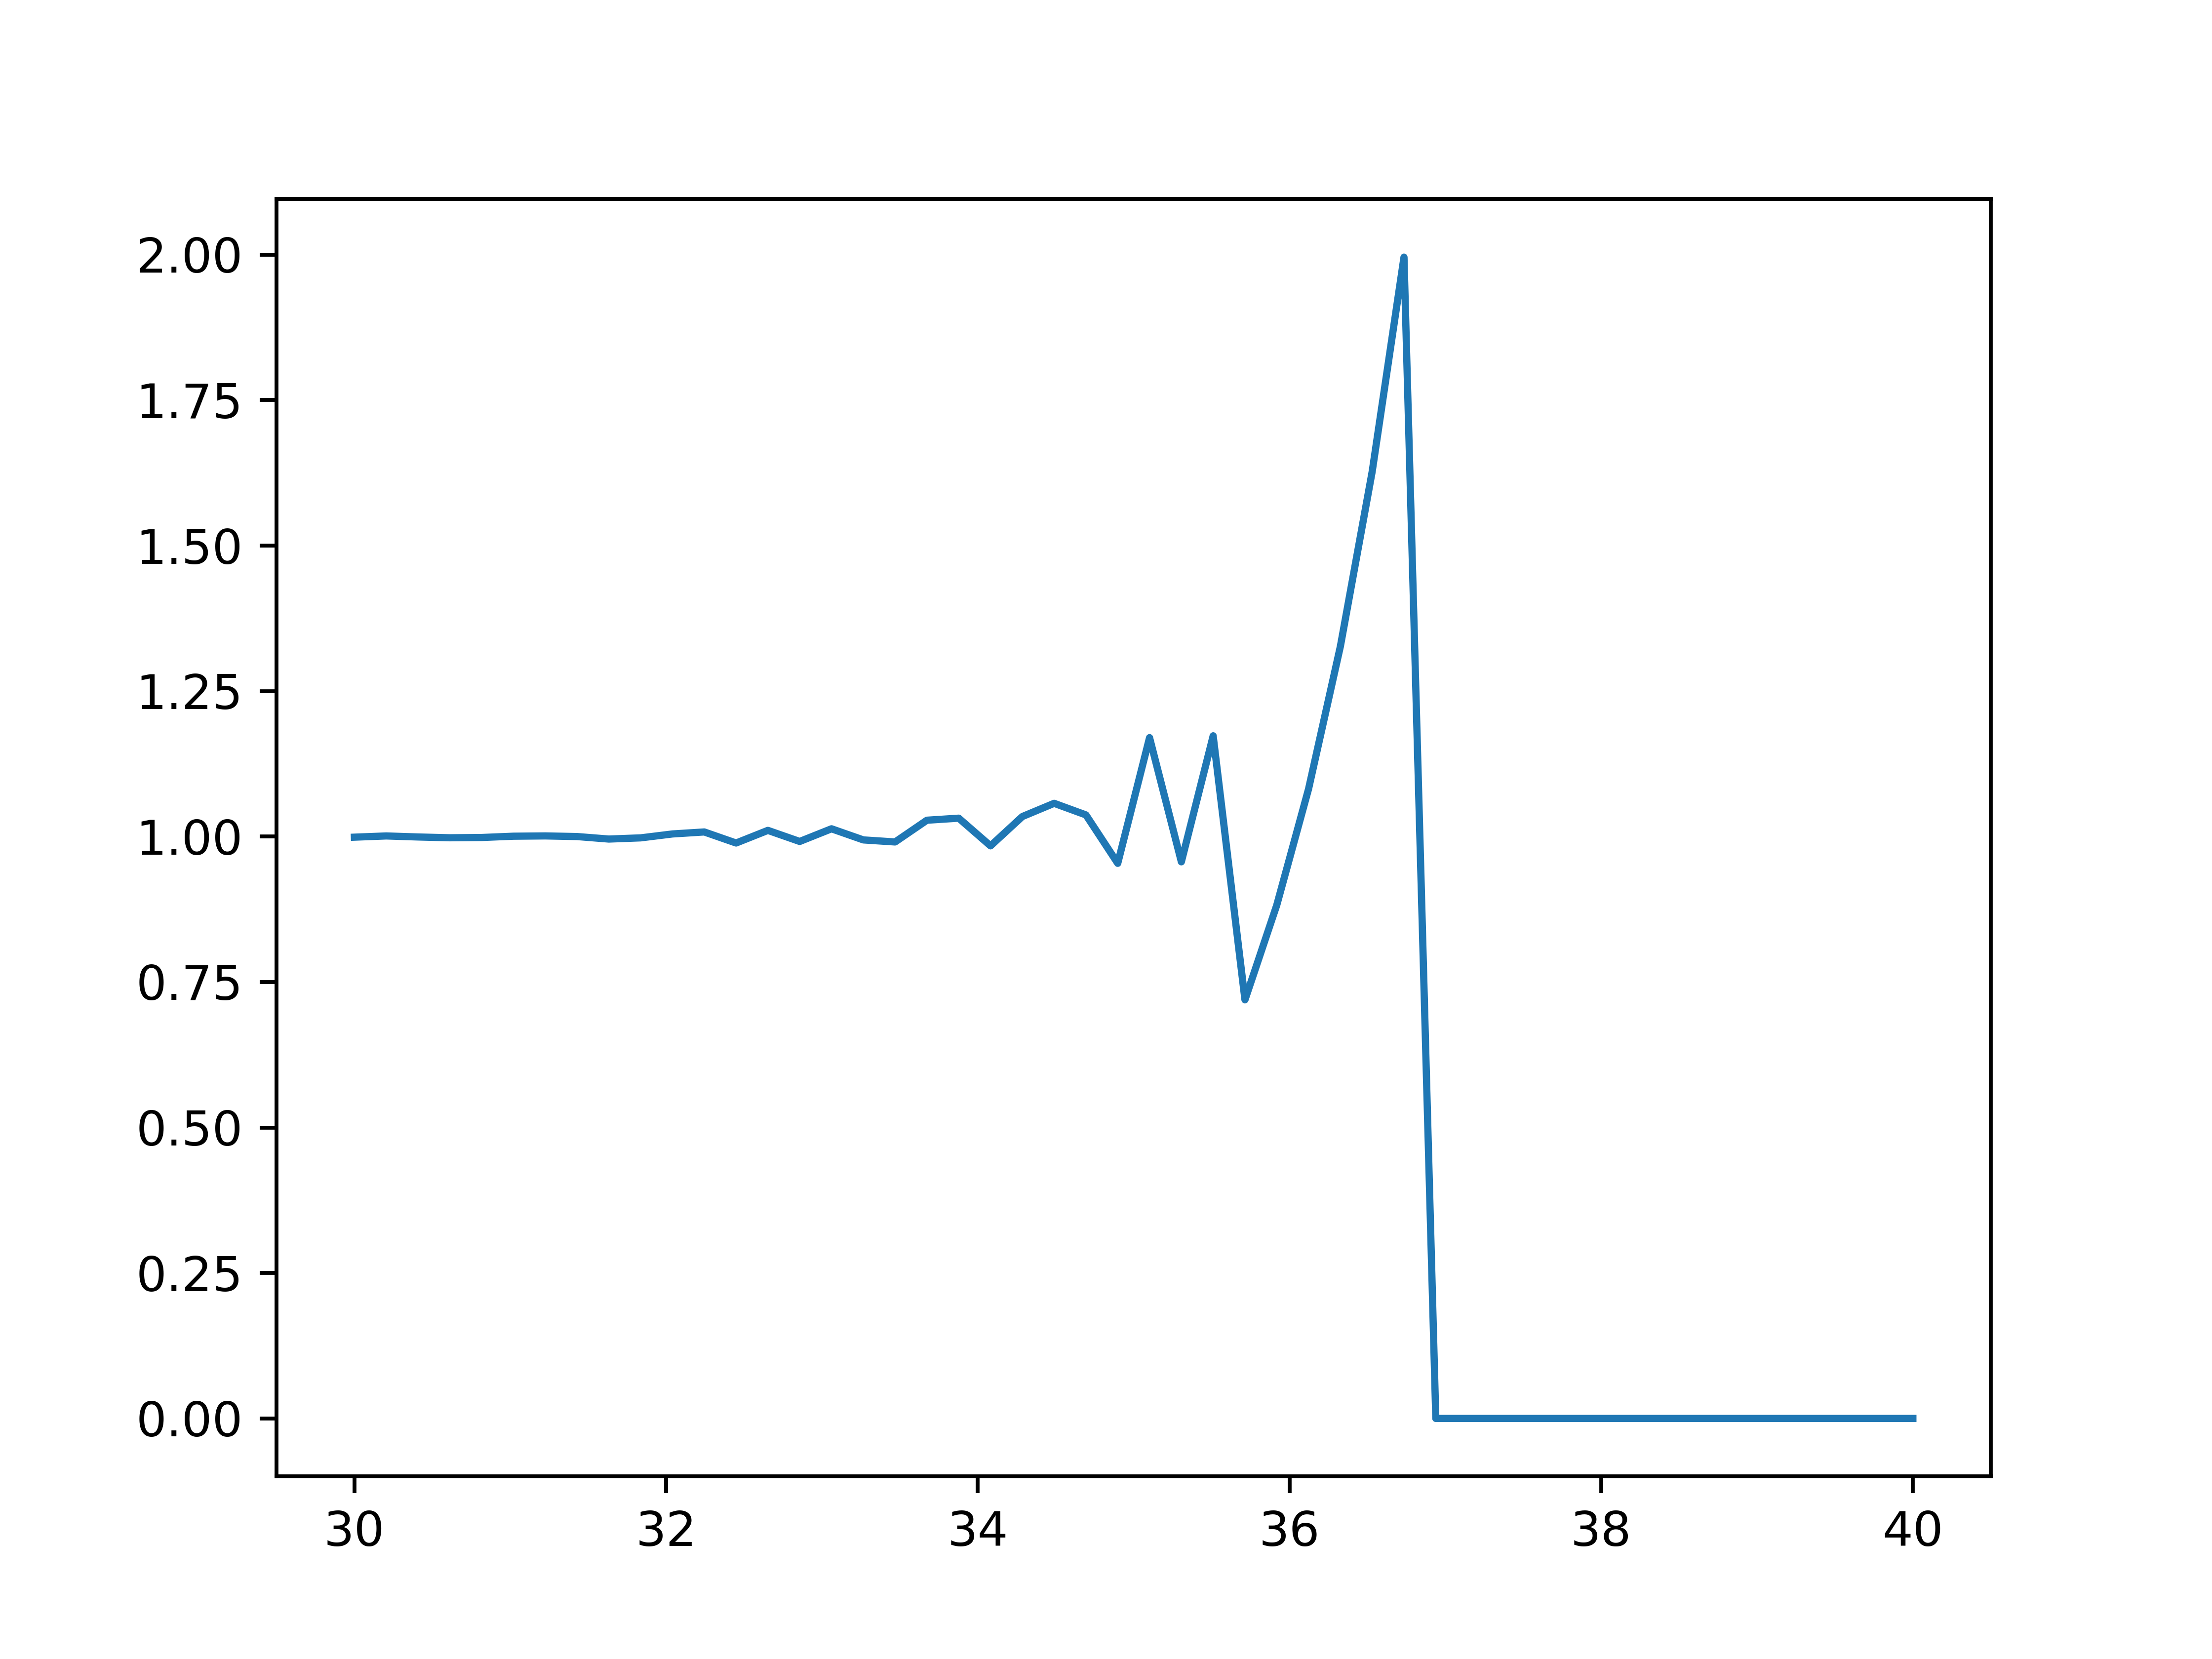
\includegraphics[width=\linewidth]{zad2_plot_py.png}
  \caption{PyPlot od 30 do 40}\label{fig:figure2}
\endminipage
\end{figure}

\begin{figure}[!htb]
\minipage{0.49\textwidth}
  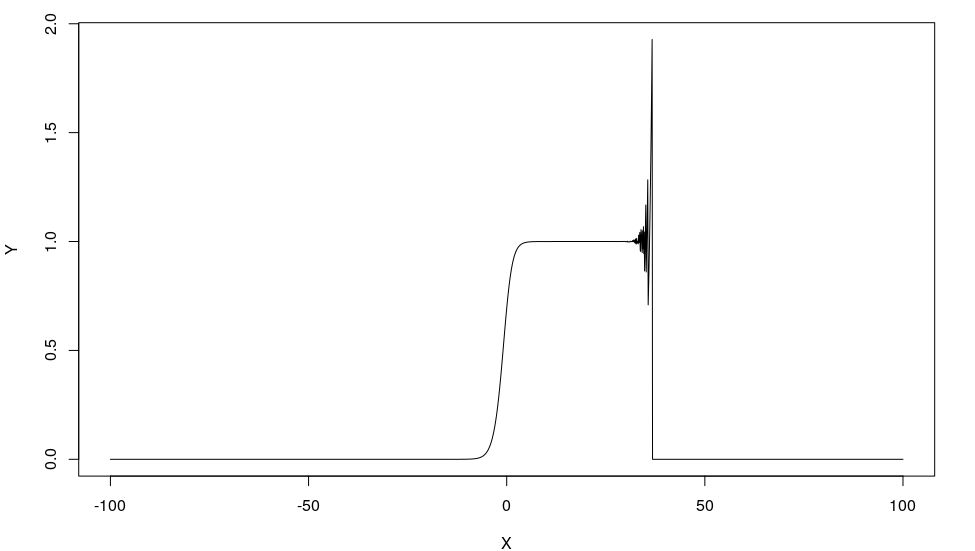
\includegraphics[width=\linewidth]{zad2_plot_2_2.jpg}
  \caption{R od -100 do 100}\label{fig:figure3}
\endminipage\hfill
\minipage{0.49\textwidth}
  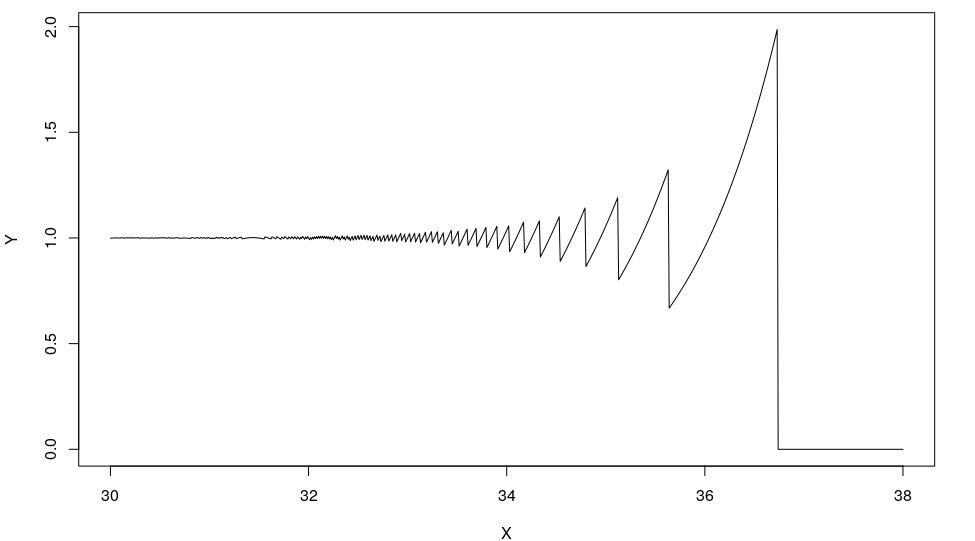
\includegraphics[width=\linewidth]{zad2_plot_3_2.jpg}
  \caption{R od 30 do 36}\label{fig:figure4}
\endminipage
\end{figure}

\subsubsection*{Granica:}
\begin{align*}
lim_{x \to \infty} e^x ln(1+e^{-x}) = lim_{x \to \infty} \frac{ln(1+e^{-x})}{e^{-x}} \stackrel{\text{z l’Hospitala}}{=} lim_{x \to \infty} \frac{-\frac{1}{e^x + 1}}{-e^{-x}} \\
= lim_{x \to \infty} \frac{e^{-x}}{e^x + 1} = lim_{x \to \infty} e^{-x} \frac{1}{lim_{x \to \infty} (e^x + 1)} = 0 \cdot 0 = 0
\end{align*}

\subsubsection*{Wnioski:}

\section{Zadanie 3}
Zadanie 3 polega na rozwiązaniu układu równań liniowych $Ax = b$ dla danej macierzy współczynników $A \in \mathbf{R}^{n \times n}$ i wektora prawych stron $b \in\mathbf{R}^{n} $.
\\
\\
\noindent Macierz $A$ generować w następujący sposób:
\begin{enumerate}
	\item{$A = H_n$, gdzie $H_n$ jest macierzą Hilberta stopnia $n$}
	\item{$A = R_n$, gdzie $R_n$ jest losową macierzą stopnia $n$ z zadanym wskaźnikiem uwarunkowania $c$}
\end{enumerate}

\noindent Wektor b zadany jest przez $b=Ax$, gdzie $A$ jest wygenerowaną macierzą, a $x = (1, ..., 1)^T$
\\
\\
\noindent Układ równań należy rozwiązać za pomocą dwóch algorytmów:
\begin{enumerate}
	\item{eliminacji Gaussa $x=A \backslash b$}
	\item{$x = A^{-1}b$}
\end{enumerate}

\noindent Eksperymenty należy wykonać dla macierzy Hilberta $H_n$ z rosnącym stopniem $n > 1$ oraz dla macierzy losowej $R_n$,$n= 5, 10, 20$ z rosnącym wskaźnikiem uwarunkowania $c = 1, 10, 10^3, 10^7, 10^{12}, 10^{16}$. Obliczony $\dot x$ należy porównać z rozwiązaniem dokładnym $x = (1, ..., 1)^T$ tj. policzyć błędy względne.
\\
\\
\noindent Wyniki przedstawiają następujące tabele:

\newpage
\begin{table}[!h]
\small
\centering
    \label{tab:table2}
    \begin{tabular}{|c|c|c|c|c|}
    		\hline
		\multicolumn{3}{|c|}{} & \multicolumn{2}{c|}{Błąd względny}\\
		\hline
		Size & Rank & Cond & Gauss & Inversion\\
\hline
2x2 & 2 & 1.928147e+01 & 5.661049e-16 & 1.404333e-15\\
\hline
3x3 & 3 & 5.240568e+02 & 8.022594e-15 & 0.000000e+00\\
\hline
4x4 & 4 & 1.551374e+04 & 4.137410e-14 & 0.000000e+00\\
\hline
5x5 & 5 & 4.766073e+05 & 1.682843e-12 & 3.354436e-12\\
\hline
6x6 & 6 & 1.495106e+07 & 2.618913e-10 & 2.016376e-10\\
\hline
7x7 & 7 & 4.753674e+08 & 1.260687e-08 & 4.713280e-09\\
\hline
8x8 & 8 & 1.525758e+10 & 6.124090e-08 & 3.077484e-07\\
\hline
9x9 & 9 & 4.931538e+11 & 3.875163e-06 & 4.541268e-06\\
\hline
10x10 & 10 & 1.602442e+13 & 8.670390e-05 & 2.501493e-04\\
\hline
11x11 & 10 & 5.222678e+14 & 1.582781e-04 & 7.618304e-03\\
\hline
12x12 & 11 & 1.751473e+16 & 1.339621e-01 & 2.589941e-01\\
\hline
13x13 & 11 & 3.344143e+18 & 1.103970e-01 & 5.331276e+00\\
\hline
14x14 & 11 & 6.200786e+17 & 1.455409e+00 & 8.714993e+00\\
\hline
15x15 & 12 & 3.674393e+17 & 4.696668e+00 & 7.344641e+00\\
\hline
16x16 & 12 & 7.865468e+17 & 5.415519e+01 & 2.984884e+01\\
\hline
17x17 & 12 & 1.263684e+18 & 1.370724e+01 & 1.051694e+01\\
\hline
18x18 & 12 & 2.244631e+18 & 9.134135e+00 & 7.575476e+00\\
\hline
19x19 & 13 & 6.471954e+18 & 9.720590e+00 & 1.223376e+01\\
\hline
20x20 & 13 & 1.355366e+18 & 7.549915e+00 & 2.206270e+01\\
\hline
    \end{tabular}
    \caption{Wartości dla macierzy Hilberta}
\end{table}

\newpage
\begin{table}[!h]
\small
\centering
    \label{tab:table3}
    \begin{tabular}{|c|c|c|c|c|}
    		\hline
		\multicolumn{3}{|c|}{} & \multicolumn{2}{c|}{Błąd względny}\\
		\hline
		Size & Rank & Cond & Gauss & Inversion\\
		\hline
5x5 & 5 & 1.000000e+00 & 1.719950e-16 & 1.216188e-16\\
\hline
10x10 & 10 & 1.000000e+00 & 1.683737e-16 & 2.482534e-16\\
\hline
20x20 & 20 & 1.000000e+00 & 6.030055e-16 & 3.358310e-16\\
\hline
5x5 & 5 & 1.000000e+01 & 7.021667e-17 & 2.275280e-16\\
\hline
10x10 & 10 & 1.000000e+01 & 5.790215e-16 & 5.135907e-16\\
\hline
20x20 & 20 & 1.000000e+01 & 7.739776e-16 & 5.628294e-16\\
\hline
5x5 & 5 & 1.000000e+03 & 5.248902e-15 & 7.399118e-15\\
\hline
10x10 & 10 & 1.000000e+03 & 2.742085e-14 & 2.134402e-14\\
\hline
20x20 & 20 & 1.000000e+03 & 2.057420e-14 & 2.385714e-14\\
\hline
5x5 & 5 & 1.000000e+07 & 4.948064e-10 & 2.472969e-10\\
\hline
10x10 & 10 & 1.000000e+07 & 3.051511e-10 & 2.871953e-10\\
\hline
20x20 & 20 & 1.000000e+07 & 2.145808e-10 & 2.235508e-10\\
\hline
5x5 & 5 & 1.000017e+12 & 1.729134e-05 & 1.722960e-05\\
\hline
10x10 & 10 & 1.000002e+12 & 3.243992e-05 & 3.472999e-05\\
\hline
20x20 & 20 & 9.999488e+11 & 1.166862e-06 & 3.780269e-06\\
\hline
5x5 & 4 & 7.861517e+15 & 2.092372e-01 & 2.078771e-01\\
\hline
10x10 & 9 & 4.124595e+16 & 1.228583e+00 & 1.310098e+00\\
\hline
20x20 & 19 & 8.132469e+15 & 4.168338e-01 & 4.414028e-01\\
\hline
    \end{tabular}
    \caption{Wartości dla losowej macierzy }
\end{table}

\subsubsection*{Wnioski:}

\section{Zadanie 4}
Zadanie 4 polega na obliczeniu 20 zer wielomianu Wilkinsona $p=(x-20)(x-19)...(x-1)$ w postaci naturalnej P i sprawdzeniu otrzymanych wyników $z_k$ obliczając wartości $|P(z_k)|$, $|p(z_k)|$ i $|z_k-k|$ dla $1 \leq k \leq 20$. Eksperyment należy powtórzyć po zaburzeniu współczynnika $-210$ na $-210-2^{-23}$. W celu rozwiązania zadanie należy użyć pakietu \textbf{Polynomials}.

\newpage
\subsubsection*{Eksperyment 1}
Otrzymane wyniki:
%\begin{lstlisting}
%[1.0, 2.0, 3.0, 4.0, 5.0, 5.99999, 7.0001, 7.99936, 9.00292, 9.99041, 11.025, 11.9533, 13.0743, 13.9148, 15.0755, 15.9463, 17.0254, 17.9909, 19.0019, 19.9998]
%\end{lstlisting}
\begin{table}[!h]
\centering
\footnotesize
    \label{tab:table4}
    \begin{tabular}{|c|c|c|c|c|}
    		\hline
    		$k$ & $z_k$ & $P(z_k)$ & $p(z_k)$ & $|z_k - k|$\\
    		\hline
1 & 1.000000e+00 & 3.635200e+04 & 5.517824e+06 & 3.010925e-13\\
\hline
2 & 2.000000e+00 & 1.817600e+05 & 7.378698e+19 & 2.831824e-11\\
\hline
3 & 3.000000e+00 & 2.094080e+05 & 3.320414e+20 & 4.079035e-10\\
\hline
4 & 4.000000e+00 & 3.106816e+06 & 8.854437e+20 & 1.626247e-08\\
\hline
5 & 5.000001e+00 & 2.411469e+07 & 1.844675e+21 & 6.657698e-07\\
\hline
6 & 5.999989e+00 & 1.201521e+08 & 3.320395e+21 & 1.075418e-05\\
\hline
7 & 7.000102e+00 & 4.803983e+08 & 5.423593e+21 & 1.020028e-04\\
\hline
8 & 7.999356e+00 & 1.682691e+09 & 8.262050e+21 & 6.441704e-04\\
\hline
9 & 9.002915e+00 & 4.465327e+09 & 1.196559e+22 & 2.915294e-03\\
\hline
10 & 9.990413e+00 & 1.270713e+10 & 1.655260e+22 & 9.586958e-03\\
\hline
11 & 1.102502e+01 & 3.575990e+10 & 2.247833e+22 & 2.502293e-02\\
\hline
12 & 1.195328e+01 & 7.216772e+10 & 2.886945e+22 & 4.671675e-02\\
\hline
13 & 1.307431e+01 & 2.157236e+11 & 3.807326e+22 & 7.431403e-02\\
\hline
14 & 1.391476e+01 & 3.653833e+11 & 4.612720e+22 & 8.524441e-02\\
\hline
15 & 1.507549e+01 & 6.139878e+11 & 5.901011e+22 & 7.549380e-02\\
\hline
16 & 1.594629e+01 & 1.555028e+12 & 7.010874e+22 & 5.371328e-02\\
\hline
17 & 1.702543e+01 & 3.777624e+12 & 8.568906e+22 & 2.542715e-02\\
\hline
18 & 1.799092e+01 & 7.199555e+12 & 1.014480e+23 & 9.078647e-03\\
\hline
19 & 1.900191e+01 & 1.027838e+13 & 1.199038e+23 & 1.909818e-03\\
\hline
20 & 1.999981e+01 & 2.746295e+13 & 1.401912e+23 & 1.907088e-04\\
\hline
    \end{tabular}
    \caption{Wartości dla oryginalnego wielomianu}
\end{table}

\newpage
\subsubsection*{Eksperyment 2}

\begin{table}[!hbt]
\centering
\footnotesize
    \label{tab:table5}
    \begin{tabular}{|c|c|c|c|c|}
    		\hline
    		$k$ & $z_k$ & $P(z_k)$ & $p(z_k)$ & $|z_k - k|$\\
		\hline
1 & 1.000000e+00 + 0.000000e+00i & 2.099200e+04 & 3.012096e+06 & 1.643130e-13\\
\hline
2 & 2.000000e+00 + 0.000000e+00i & 3.491840e+05 & 7.378698e+19 & 5.503731e-11\\
\hline
3 & 3.000000e+00 + 0.000000e+00i & 2.221568e+06 & 3.320414e+20 & 3.396580e-09\\
\hline
4 & 4.000000e+00 + 0.000000e+00i & 1.046784e+07 & 8.854438e+20 & 8.972436e-08\\
\hline
5 & 4.999999e+00 + 0.000000e+00i & 3.946394e+07 & 1.844673e+21 & 1.426112e-06\\
\hline
6 & 6.000020e+00 + 0.000000e+00i & 1.291484e+08 & 3.320450e+21 & 2.047667e-05\\
\hline
7 & 6.999602e+00 + 0.000000e+00i & 3.881231e+08 & 5.422367e+21 & 3.979296e-04\\
\hline
8 & 8.007772e+00 + 0.000000e+00i & 1.072547e+09 & 8.289400e+21 & 7.772029e-03\\
\hline
9 & 8.915816e+00 + 0.000000e+00i & 3.065575e+09 & 1.160747e+22 & 8.418363e-02\\
\hline
10 & 1.009546e+01 + -6.449328e-01i & 7.143114e+09 & 1.721289e+22 & 6.519587e-01\\
\hline
11 & 1.009546e+01 + 6.449328e-01i & 7.143114e+09 & 1.721289e+22 & 1.110918e+00\\
\hline
12 & 1.179389e+01 + -1.652477e+00i & 3.357756e+10 & 2.856840e+22 & 1.665281e+00\\
\hline
13 & 1.179389e+01 + 1.652477e+00i & 3.357756e+10 & 2.856840e+22 & 2.045820e+00\\
\hline
14 & 1.399241e+01 + -2.518824e+00i & 1.061206e+11 & 4.934647e+22 & 2.518836e+00\\
\hline
15 & 1.399241e+01 + 2.518824e+00i & 1.061206e+11 & 4.934647e+22 & 2.712881e+00\\
\hline
16 & 1.673074e+01 + -2.812625e+00i & 3.315103e+11 & 8.484695e+22 & 2.906002e+00\\
\hline
17 & 1.673074e+01 + 2.812625e+00i & 3.315103e+11 & 8.484695e+22 & 2.825484e+00\\
\hline
18 & 1.950244e+01 + -1.940332e+00i & 9.539425e+12 & 1.318195e+23 & 2.454021e+00\\
\hline
19 & 1.950244e+01 + 1.940332e+00i & 9.539425e+12 & 1.318195e+23 & 2.004329e+00\\
\hline
20 & 2.084691e+01 + 0.000000e+00i & 1.114454e+13 & 1.591108e+23 & 8.469102e-01\\
\hline
    \end{tabular}
    \caption{Wartości dla zmodyfikowanego wielomianu}
\end{table}

\subsubsection*{Wnioski:}

\section{Zadanie 5}
W zadaniu 5 rozważamy równanie rekurencyjne przedstawiające model wzrostu populacji:
\begin{equation*}
	p_{n+1} := p_n+rp_n(1-p_n)
\end{equation*}
gdzie $r$ jest pewną daną stałą, $r(1-p_n)$ jest czynnikiem wzrostu populacji, a $p_0$ jest wielkością populacji stanowiąca procent maksymalnej wielkości populacji dla danego stanu środowiska.

Należy przeprowadzić następujące eksperymenty:
\begin{enumerate}
	\item{Dla danych $p_0 = 0.01$ i $r = 3$ wykonać 40 iteracji wyrażenia, a następnie wykonać ponownie 40 iteracji wyrażenia z niewielką modyfikacją tj. wykonać 10 iteracji, zatrzymać, zastosować obcięcie wyniku odrzucając cyfry po trzecim miejscu po przecinku i kontynuować dalej obliczenia. Porównać otrzymane wyniki.}
	\item{Dla danych $p_0 = 0.01$ i $r = 3$ wykonać 40 iteracji wyrażenia w arytmetyce \textbf{Float32} i \textbf{Float64}. Porównać otrzymane wyniki.}
\end{enumerate}

Wyniki przedstawiam w poniższych tabelach:

\begin{table}[!hbt]
\centering
\footnotesize
    \label{tab:table6}
    \begin{tabular}{|c|c|c|}
    		\hline
    		& \multicolumn{2}{|c|}{$p_n$} \\
    		\hline
    		$n$ & przed mod. & po mod.\\
    		\hline
		\hline
1 & 0.0397 & 0.0397\\
\hline
2 & 0.15407173 & 0.15407173\\
\hline
3 & 0.5450726 & 0.5450726\\
\hline
4 & 1.2889781 & 1.2889781\\
\hline
5 & 0.1715188 & 0.1715188\\
\hline
\hline
10 & 0.7229306 & 0.722\\
\hline
15 & 1.2704837 & 1.2572169\\
\hline
20 & 0.5799036 & 1.3096911\\
\hline
25 & 1.0070806 & 1.0929108\\
\hline
30 & 0.7529209 & 1.3191822\\
\hline
\hline
35 & 1.021099 & 0.034241438\\
\hline
36 & 0.95646656 & 0.13344833\\
\hline
37 & 1.0813814 & 0.48036796\\
\hline
38 & 0.81736827 & 1.2292118\\
\hline
39 & 1.2652004 & 0.3839622\\
\hline
40 & 0.25860548 & 1.093568\\
\hline
    \end{tabular}
    \caption{Wartości dla eksperymentu 1}
\end{table}

\begin{table}[!hbt]
\centering
\footnotesize
    \label{tab:table7}
    \begin{tabular}{|c|c|c|}
    		\hline
    		 & \multicolumn{2}{c|}{$p_n$} \\
    		 \hline
    		 $n$ & Float32 & Float64\\
    		\hline
    		\hline
1 & 0.0397 & 0.0397\\
\hline
2 & 0.15407173 & 0.15407173000000002\\
\hline
3 & 0.5450726 & 0.5450726260444213\\
\hline
4 & 1.2889781 & 1.2889780011888006\\
\hline
5 & 0.1715188 & 0.17151914210917552\\
\hline
\hline
10 & 0.7229306 & 0.722914301179573\\
\hline
15 & 1.2704837 & 1.2702617739350768\\
\hline
20 & 0.5799036 & 0.5965293124946907\\
\hline
25 & 1.0070806 & 1.315588346001072\\
\hline
30 & 0.7529209 & 0.37414648963928676\\
\hline
\hline
35 & 1.021099 & 0.9253821285571046\\
\hline
36 & 0.95646656 & 1.1325322626697856\\
\hline
37 & 1.0813814 & 0.6822410727153098\\
\hline
38 & 0.81736827 & 1.3326056469620293\\
\hline
39 & 1.2652004 & 0.0029091569028512065\\
\hline
40 & 0.25860548 & 0.011611238029748606\\
\hline
    \end{tabular}
    \caption{Wartości dla eksperymentu 2}
\end{table}

Powyższe dane w formie wykresów:
%\begin{figure}[!htb]
%  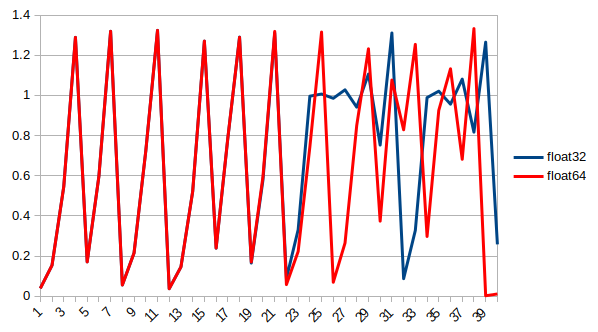
\includegraphics[width=\linewidth]{plot_zad5_1.png}
%  \caption{Eksperyment 1}
%  \label{fig:figure4}
%\end{figure}
%\begin{figure}[!htb]
%  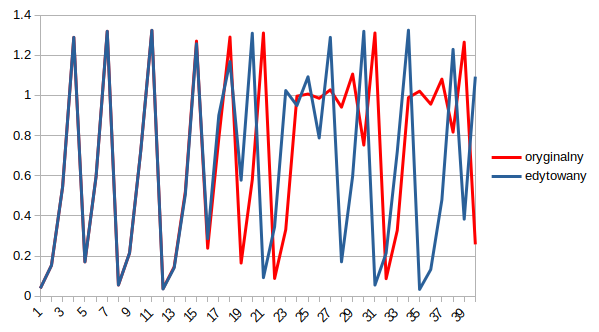
\includegraphics[width=\linewidth]{plot_zad5_2.png}
%  \caption{Eksperyment 2}
%  \label{fig:figure5}
%\end{figure}

\newpage
\subsubsection*{Wnioski:}

\section{Zadanie 6}
W zadaniu 6 rozważamy równanie rekurencyjne:
\begin{equation*}
	x_{n+1} := x_n^2 + c
\end{equation*} 
gdzie $c$ jest pewną stałą.
\\
\\
\noindent Należy przeprowadzić następujące eksperymenty. Dla danych: 
\begin{enumerate}
	\item{$c = -2$ i $x_0 = 1$}
	\item{$c = -2$ i $x_0 = 2$}
	\item{$c = -2$ i $x_0 = 1.99999999999999$}
	\item{$c = -1$ i $x_0 = 1$}
	\item{$c = -1$ i $x_0 = -1$}
	\item{$c = -1$ i $x_0 = 0.75$}
	\item{$c = -1$ i $x_0 = 0.25$}
\end{enumerate}
wykonać w języku \textbf{Julia} w arytmetyce \textbf{Float64} 40 iteracji wyrażania oraz zaobserwować zachowanie generowanych ciągów.

Uzyskane wartości przedstawiają następujące wykresy:

\begin{figure}[!htb]
\minipage{0.49\textwidth}
  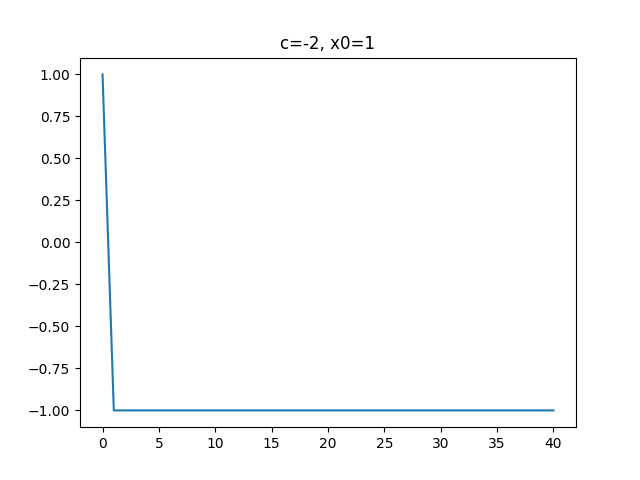
\includegraphics[width=\linewidth]{1.png}
  \caption{Eksperyment 1}
\endminipage\hfill
\minipage{0.49\textwidth}
  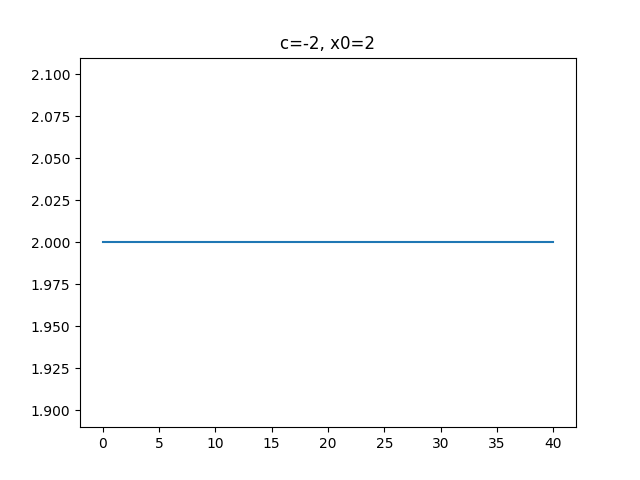
\includegraphics[width=\linewidth]{2.png}
  \caption{Eksperyment 2}
\endminipage
\end{figure}

\newpage
\begin{figure}[!htb]
\minipage{0.49\textwidth}
  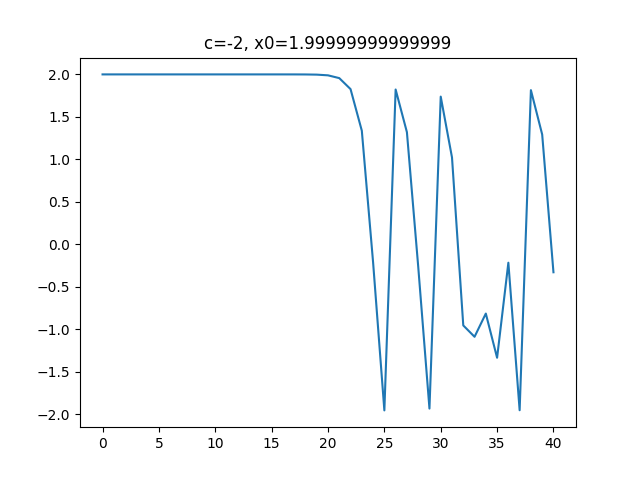
\includegraphics[width=\linewidth]{3.png}
  \caption{Eksperyment 3}
\endminipage\hfill
\minipage{0.49\textwidth}
  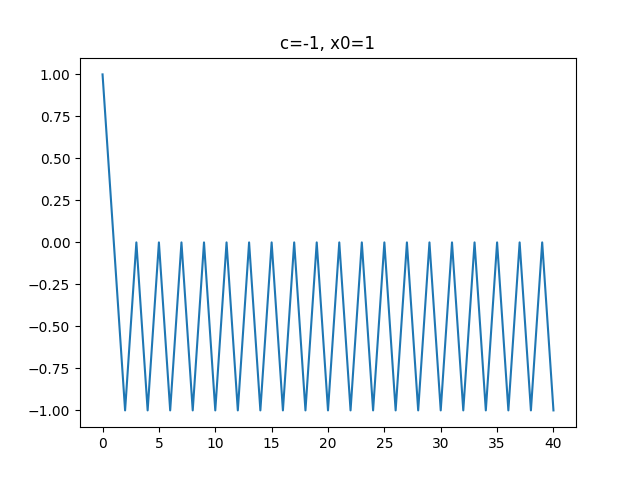
\includegraphics[width=\linewidth]{4.png}
  \caption{Eksperyment 4}
\endminipage
\end{figure}

\begin{figure}[!htb]
\minipage{0.49\textwidth}
  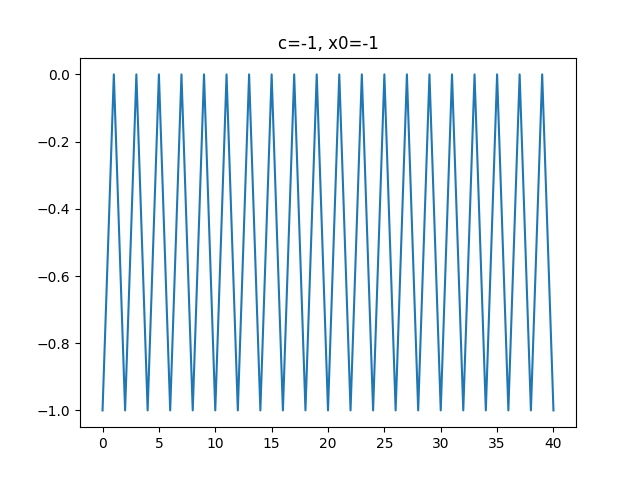
\includegraphics[width=\linewidth]{5.png}
  \caption{Eksperyment 5}
\endminipage\hfill
\minipage{0.49\textwidth}
  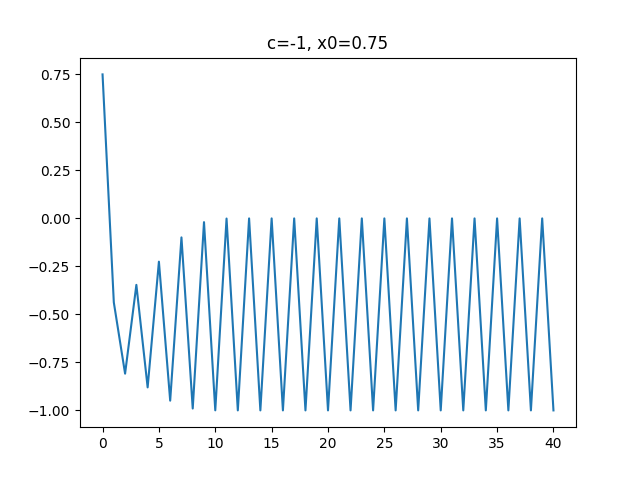
\includegraphics[width=\linewidth]{6.png}
  \caption{Eksperyment 6}
\endminipage
\end{figure}

\newpage
\begin{figure}[!hbt]
	\centering
	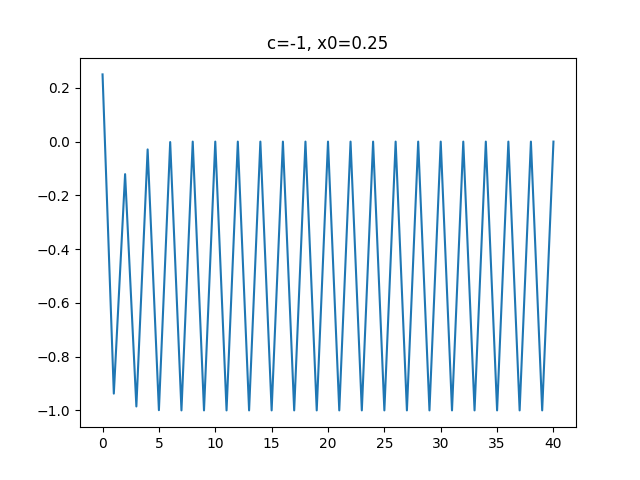
\includegraphics[width=0.6\linewidth]{7.png}
  \caption{Eksperyment 7}
\end{figure}

\newpage
\begin{table}[!h]
\centering
\footnotesize
    \label{tab:table8}
    \begin{tabular}{|c|c|c|c|c|c|c|c|}
    		\hline
    		$n$ & \multicolumn{3}{|c|}{$c=-2$} & \multicolumn{4}{|c|}{$c=-1$}\\
    		\hline
    		$x_0=1$ & $x_0=2$ & $x_0=1.99[...]$ & $x_0=1$ & $x_0=-1$ & $x_0=0.75$ & $x_0=0.25$\\
    		\hline
0 & 1.0 & 2.0 & 2.000000e+00 & 1.0 & -1.0 & 7.500000e-01 & 2.500000e-01\\
\hline
1 & -1.0 & 2.0 & 2.000000e+00 & 0.0 & 0.0 & -4.375000e-01 & -9.375000e-01\\
\hline
2 & -1.0 & 2.0 & 2.000000e+00 & -1.0 & -1.0 & -8.085938e-01 & -1.210938e-01\\
\hline
3 & -1.0 & 2.0 & 2.000000e+00 & 0.0 & 0.0 & -3.461761e-01 & -9.853363e-01\\
\hline
4 & -1.0 & 2.0 & 2.000000e+00 & -1.0 & -1.0 & -8.801621e-01 & -2.911237e-02\\
\hline
5 & -1.0 & 2.0 & 2.000000e+00 & 0.0 & 0.0 & -2.253147e-01 & -9.991525e-01\\
\hline
6 & -1.0 & 2.0 & 2.000000e+00 & -1.0 & -1.0 & -9.492333e-01 & -1.694342e-03\\
\hline
7 & -1.0 & 2.0 & 2.000000e+00 & 0.0 & 0.0 & -9.895619e-02 & -9.999971e-01\\
\hline
8 & -1.0 & 2.0 & 2.000000e+00 & -1.0 & -1.0 & -9.902077e-01 & -5.741579e-06\\
\hline
9 & -1.0 & 2.0 & 2.000000e+00 & 0.0 & 0.0 & -1.948876e-02 & -1.000000e+00\\
\hline
10 & -1.0 & 2.0 & 2.000000e+00 & -1.0 & -1.0 & -9.996202e-01 & -6.593148e-11\\
\hline
11 & -1.0 & 2.0 & 2.000000e+00 & 0.0 & 0.0 & -7.594796e-04 & -1.000000e+00\\
\hline
12 & -1.0 & 2.0 & 2.000000e+00 & -1.0 & -1.0 & -9.999994e-01 & 0.000000e+00\\
\hline
13 & -1.0 & 2.0 & 1.999999e+00 & 0.0 & 0.0 & -1.153618e-06 & -1.000000e+00\\
\hline
14 & -1.0 & 2.0 & 1.999997e+00 & -1.0 & -1.0 & -1.000000e+00 & 0.000000e+00\\
\hline
15 & -1.0 & 2.0 & 1.999989e+00 & 0.0 & 0.0 & -2.661649e-12 & -1.000000e+00\\
\hline
16 & -1.0 & 2.0 & 1.999957e+00 & -1.0 & -1.0 & -1.000000e+00 & 0.000000e+00\\
\hline
17 & -1.0 & 2.0 & 1.999828e+00 & 0.0 & 0.0 & 0.000000e+00 & -1.000000e+00\\
\hline
18 & -1.0 & 2.0 & 1.999313e+00 & -1.0 & -1.0 & -1.000000e+00 & 0.000000e+00\\
\hline
19 & -1.0 & 2.0 & 1.997254e+00 & 0.0 & 0.0 & 0.000000e+00 & -1.000000e+00\\
\hline
20 & -1.0 & 2.0 & 1.989024e+00 & -1.0 & -1.0 & -1.000000e+00 & 0.000000e+00\\
\hline
21 & -1.0 & 2.0 & 1.956215e+00 & 0.0 & 0.0 & 0.000000e+00 & -1.000000e+00\\
\hline
22 & -1.0 & 2.0 & 1.826779e+00 & -1.0 & -1.0 & -1.000000e+00 & 0.000000e+00\\
\hline
23 & -1.0 & 2.0 & 1.337120e+00 & 0.0 & 0.0 & 0.000000e+00 & -1.000000e+00\\
\hline
24 & -1.0 & 2.0 & -2.121097e-01 & -1.0 & -1.0 & -1.000000e+00 & 0.000000e+00\\
\hline
25 & -1.0 & 2.0 & -1.955009e+00 & 0.0 & 0.0 & 0.000000e+00 & -1.000000e+00\\
\hline
26 & -1.0 & 2.0 & 1.822062e+00 & -1.0 & -1.0 & -1.000000e+00 & 0.000000e+00\\
\hline
27 & -1.0 & 2.0 & 1.319910e+00 & 0.0 & 0.0 & 0.000000e+00 & -1.000000e+00\\
\hline
28 & -1.0 & 2.0 & -2.578368e-01 & -1.0 & -1.0 & -1.000000e+00 & 0.000000e+00\\
\hline
29 & -1.0 & 2.0 & -1.933520e+00 & 0.0 & 0.0 & 0.000000e+00 & -1.000000e+00\\
\hline
30 & -1.0 & 2.0 & 1.738500e+00 & -1.0 & -1.0 & -1.000000e+00 & 0.000000e+00\\
\hline
31 & -1.0 & 2.0 & 1.022383e+00 & 0.0 & 0.0 & 0.000000e+00 & -1.000000e+00\\
\hline
32 & -1.0 & 2.0 & -9.547330e-01 & -1.0 & -1.0 & -1.000000e+00 & 0.000000e+00\\
\hline
33 & -1.0 & 2.0 & -1.088485e+00 & 0.0 & 0.0 & 0.000000e+00 & -1.000000e+00\\
\hline
34 & -1.0 & 2.0 & -8.152007e-01 & -1.0 & -1.0 & -1.000000e+00 & 0.000000e+00\\
\hline
35 & -1.0 & 2.0 & -1.335448e+00 & 0.0 & 0.0 & 0.000000e+00 & -1.000000e+00\\
\hline
36 & -1.0 & 2.0 & -2.165791e-01 & -1.0 & -1.0 & -1.000000e+00 & 0.000000e+00\\
\hline
37 & -1.0 & 2.0 & -1.953094e+00 & 0.0 & 0.0 & 0.000000e+00 & -1.000000e+00\\
\hline
38 & -1.0 & 2.0 & 1.814574e+00 & -1.0 & -1.0 & -1.000000e+00 & 0.000000e+00\\
\hline
39 & -1.0 & 2.0 & 1.292680e+00 & 0.0 & 0.0 & 0.000000e+00 & -1.000000e+00\\
\hline
40 & -1.0 & 2.0 & -3.289791e-01 & -1.0 & -1.0 & -1.000000e+00 & 0.000000e+00\\
\hline
    	    \end{tabular}
    \caption{Wartości z zadania 6}
\end{table}
\newpage
\subsubsection*{Wnioski:}
blah blah blah blah blah blah blah blah 
blah blah blah blah blah blah blah blah 
blah blah blah blah blah blah blah blah 
blah blah blah blah blah blah blah blah 
blah blah blah blah blah blah blah blah 
blah blah blah blah blah blah blah blah 
blah blah blah blah blah blah blah blah 
blah blah blah blah blah blah blah blah 
blah blah blah blah blah blah blah blah 
blah blah blah blah blah blah blah blah 
blah blah blah blah blah blah blah blah 
blah blah blah blah blah blah blah blah 
blah blah blah blah blah blah blah blah 
blah blah blah blah blah blah blah blah 
blah blah blah blah blah blah blah blah 
blah blah blah blah blah blah blah blah 
blah blah blah blah blah blah blah blah 
blah blah blah blah blah blah blah blah 


\end{document}